%----------------------------------------------------------------------------------------
%
% A LaTeX-template for 1DV510. Modified and translated by Björn Lindenberg at LNU.
% Based on an original master thesis template created by Marcus Wilhelmsson at LNU.
%
%----------------------------------------------------------------------------------------

% Settings and document configuration

\documentclass[a4paper,12pt]{article} 
\usepackage[T1]{fontenc} 
\usepackage{times} 
\usepackage[swedish,english]{babel} 
\usepackage[utf8]{inputenc} 
\usepackage{dtk-logos} 
\usepackage{wallpaper} 
\usepackage[absolute]{textpos} 
\usepackage[top=2cm, bottom=2.5cm, left=3cm, right=3cm]{geometry} 
\usepackage[parfill]{parskip} 
\usepackage{csquotes} 
\usepackage{float} 
\usepackage{lipsum} % Used for dummy text. Can be removed.
\usepackage{listings, color}
\lstdefinestyle{Asm}{
  belowcaptionskip=1\baselineskip,
  breaklines=true,
  frame=L,
  xleftmargin=\parindent,
  language=[x86masm]Assembler,
  showstringspaces=false,
  basicstyle=\footnotesize\ttfamily,
  keywordstyle=\bfseries\color{purple!40!black},
  commentstyle=\itshape\color{green!40!black},
  identifierstyle=\color{blue},
  stringstyle=\color{orange},
}

% Fontsizes for section headings.
\usepackage{sectsty} 
\sectionfont{\fontsize{14}{15}\selectfont}
\subsectionfont{\fontsize{12}{15}\selectfont}
\subsubsectionfont{\fontsize{12}{15}\selectfont}

%----------------------------------------------------------------------------------------
%	This part is used for the text box on the title page
%----------------------------------------------------------------------------------------
\newsavebox{\mybox}
\newlength{\mydepth}
\newlength{\myheight}

\newenvironment{sidebar}%
{\begin{lrbox}{\mybox}\begin{minipage}{\textwidth}}%
{\end{minipage}\end{lrbox}%
 \settodepth{\mydepth}{\usebox{\mybox}}%
 \settoheight{\myheight}{\usebox{\mybox}}%
 \addtolength{\myheight}{\mydepth}%
 \noindent\makebox[0pt]{\hspace{-20pt}\rule[-\mydepth]{1pt}{\myheight}}%
 \usebox{\mybox}}

%----------------------------------------------------------------------------------------
%	Title
%----------------------------------------------------------------------------------------
\newcommand\BackgroundPic{
    \put(-2,-3){
    
\includegraphics[keepaspectratio,scale=0.3]{img/lnu_etch.png} % Background image
    }
}
\newcommand\BackgroundPicLogo{
    \put(30,740){
    
\includegraphics[keepaspectratio,scale=0.10]{img/logo.png} % LNU logo
    }
}

\title{
\vspace{-8cm}
\begin{sidebar}
    \vspace{10cm}
    \normalfont \normalsize
    \huge Computer Technology I\\ % Main title
    \vspace{-1.3cm}
\end{sidebar}
\vspace{3cm}
\begin{flushleft}
    \huge Lab. 5 : Display JHD202 % Subtitle
     \small \\ \emph{}
\end{flushleft}
\null
\vfill
\begin{textblock}{5}(10,13)
\begin{flushright}
\begin{minipage}{\textwidth}
\begin{flushleft} \large
\emph{Author:}\textsc{Anas Kwefati}\\  % Author
\emph{Supervisor:}  \textsc{Anders Haggren} \\  % Author
\emph{Semester:} Autumn 2019\\ % Semester
\emph{Area:} Computer Science \\ % Area
\emph{Course code:} 1DT301 % Course
\end{flushleft}
\end{minipage}
\end{flushright}
\end{textblock}
}

\date{} % Empty date command. Use \today inside for today's date.
\author{} % Normally one would use this to define authors. However in this case the title command takes care of everything, so we leave the field empty to get rid of warnings. 

\begin{document}

\pagenumbering{gobble} % Turn off page numbering
\newgeometry{left=5cm}
\AddToShipoutPicture*{\BackgroundPic} % Adds the background image to the title page
\AddToShipoutPicture*{\BackgroundPicLogo} % Adds the logo to the title page
\maketitle % Prints the title
\restoregeometry
\clearpage

\pagenumbering{roman} % Roman page numbering for abstract page


\selectlanguage{english}

\newpage

\pagenumbering{gobble} % Turn off page numbering
\tableofcontents 

\newpage
\pagenumbering{arabic} % Turn on page numbering

%TASK1
\section{Task 1}
\lstset{style=Asm}

\begin{lstlisting}
;>>>>>>>>>>>>>>>>>>>>>>>>>>>>>>>>>>>>>>>>>>>>>>>>>>>>>>>>>>>
; 1DT301, Computer Technology I
; Date: 2016-09-15
; Author:
;	Anas Kwefati
;
; Lab number: 5
; Title: Display JHD202
;
; Hardware: STK600, CPU ATmega2560
;
; Function: Program that displays the character %.
;
; Input ports: none
;
; Output ports: LCD JHD202 on PORTE.
;
; Subroutines:
; Included files: m2560def.inc
;
; Other information: The program lab5_init_display.asm was used
; Changes in program: (Description and date)
;<<<<<<<<<<<<<<<<<<<<<<<<<<<<<<<<<<<<<<<<<<<<<<<<<<<<<<<<<<<

.include 	"m2560def.inc"
.def	Temp	= r16
.def	Data	= r17
.def	RS	= r18

.equ	BITMODE4	= 0b00000010		; 4-bit operation
.equ	CLEAR	= 0b00000001			; Clear display
.equ	DISPCTRL	= 0b00001111		; Display on, cursor on, blink on.

.cseg
.org	0x0000				; Reset vector
	jmp reset

.org	0x0072

reset:

	ldi Temp, HIGH(RAMEND)	; Temp = high byte of ramend address
	out SPH, Temp			; sph = Temp
	ldi Temp, LOW(RAMEND)	; Temp = low byte of ramend address
	out SPL, Temp			; spl = Temp

	ser Temp				; r16 = 0b11111111
	out DDRE, Temp			; port E = outputs ( Display JHD202A)
	clr Temp				; r16 = 0
	out PORTE, Temp

	;DISPLAY % CHARACTER
	rcall init_disp ;We call init_disp to initialize the display
	ldi data, '%' ;Set the character % to Data (r17)
	rcall write_char ;Call write_char that will convert % to binary code to display it

loop:	nop
	rjmp loop			; loop forever

; **
; ** init_display
; **
init_disp:
	rcall power_up_wait		; wait for display to power up

	ldi Data, BITMODE4		; 4-bit operation
	rcall write_nibble		; (in 8-bit mode)
	rcall short_wait		; wait min. 39 us
	ldi Data, DISPCTRL		; disp. on, blink on, curs. On
	rcall write_cmd			; send command
	rcall short_wait		; wait min. 39 us
clr_disp:
	ldi Data, CLEAR			; clr display
	rcall write_cmd			; send command
	rcall long_wait			; wait min. 1.53 ms
	ret

; **
; ** write char/command
; **

write_char:
	ldi RS, 0b00100000		; RS = high
	rjmp write
write_cmd:
	clr RS					; RS = low
write:
	mov Temp, Data			; copy Data
	andi Data, 0b11110000	; mask out high nibble
	swap Data				; swap nibbles
	or Data, RS				; add register select
	rcall write_nibble		; send high nibble
	mov Data, Temp			; restore Data
	andi Data, 0b00001111	; mask out low nibble
	or Data, RS				; add register select

write_nibble:
	rcall switch_output		; Modify for display JHD202A, port E
	nop						; wait 542nS
	sbi PORTE, 5			; enable high, JHD202A
	nop
	nop						; wait 542nS
	cbi PORTE, 5			; enable low, JHD202A
	nop
	nop						; wait 542nS
	ret

; **
; ** busy_wait loop
; **
short_wait:
	clr zh					; approx 50 us
	ldi zl, 30
	rjmp wait_loop
long_wait:
	ldi zh, HIGH(1000)		; approx 2 ms
	ldi zl, LOW(1000)
	rjmp wait_loop
dbnc_wait:
	ldi zh, HIGH(4600)		; approx 10 ms
	ldi zl, LOW(4600)
	rjmp wait_loop
power_up_wait:
	ldi zh, HIGH(9000)		; approx 20 ms
	ldi zl, LOW(9000)

wait_loop:
	sbiw z, 1				; 2 cycles
	brne wait_loop			; 2 cycles
	ret

; **
; ** modify output signal to fit LCD JHD202A, connected to port E
; **

switch_output:
	push Temp
	clr Temp
	sbrc Data, 0				; D4 = 1?
	ori Temp, 0b00000100		; Set pin 2
	sbrc Data, 1				; D5 = 1?
	ori Temp, 0b00001000		; Set pin 3
	sbrc Data, 2				; D6 = 1?
	ori Temp, 0b00000001		; Set pin 0
	sbrc Data, 3				; D7 = 1?
	ori Temp, 0b00000010		; Set pin 1
	sbrc Data, 4				; E = 1?
	ori Temp, 0b00100000		; Set pin 5
	sbrc Data, 5				; RS = 1?
	ori Temp, 0b10000000		; Set pin 7 (wrong in previous version)
	out porte, Temp
	pop Temp
	ret


\end{lstlisting}


\begin{figure}
\begin{center}
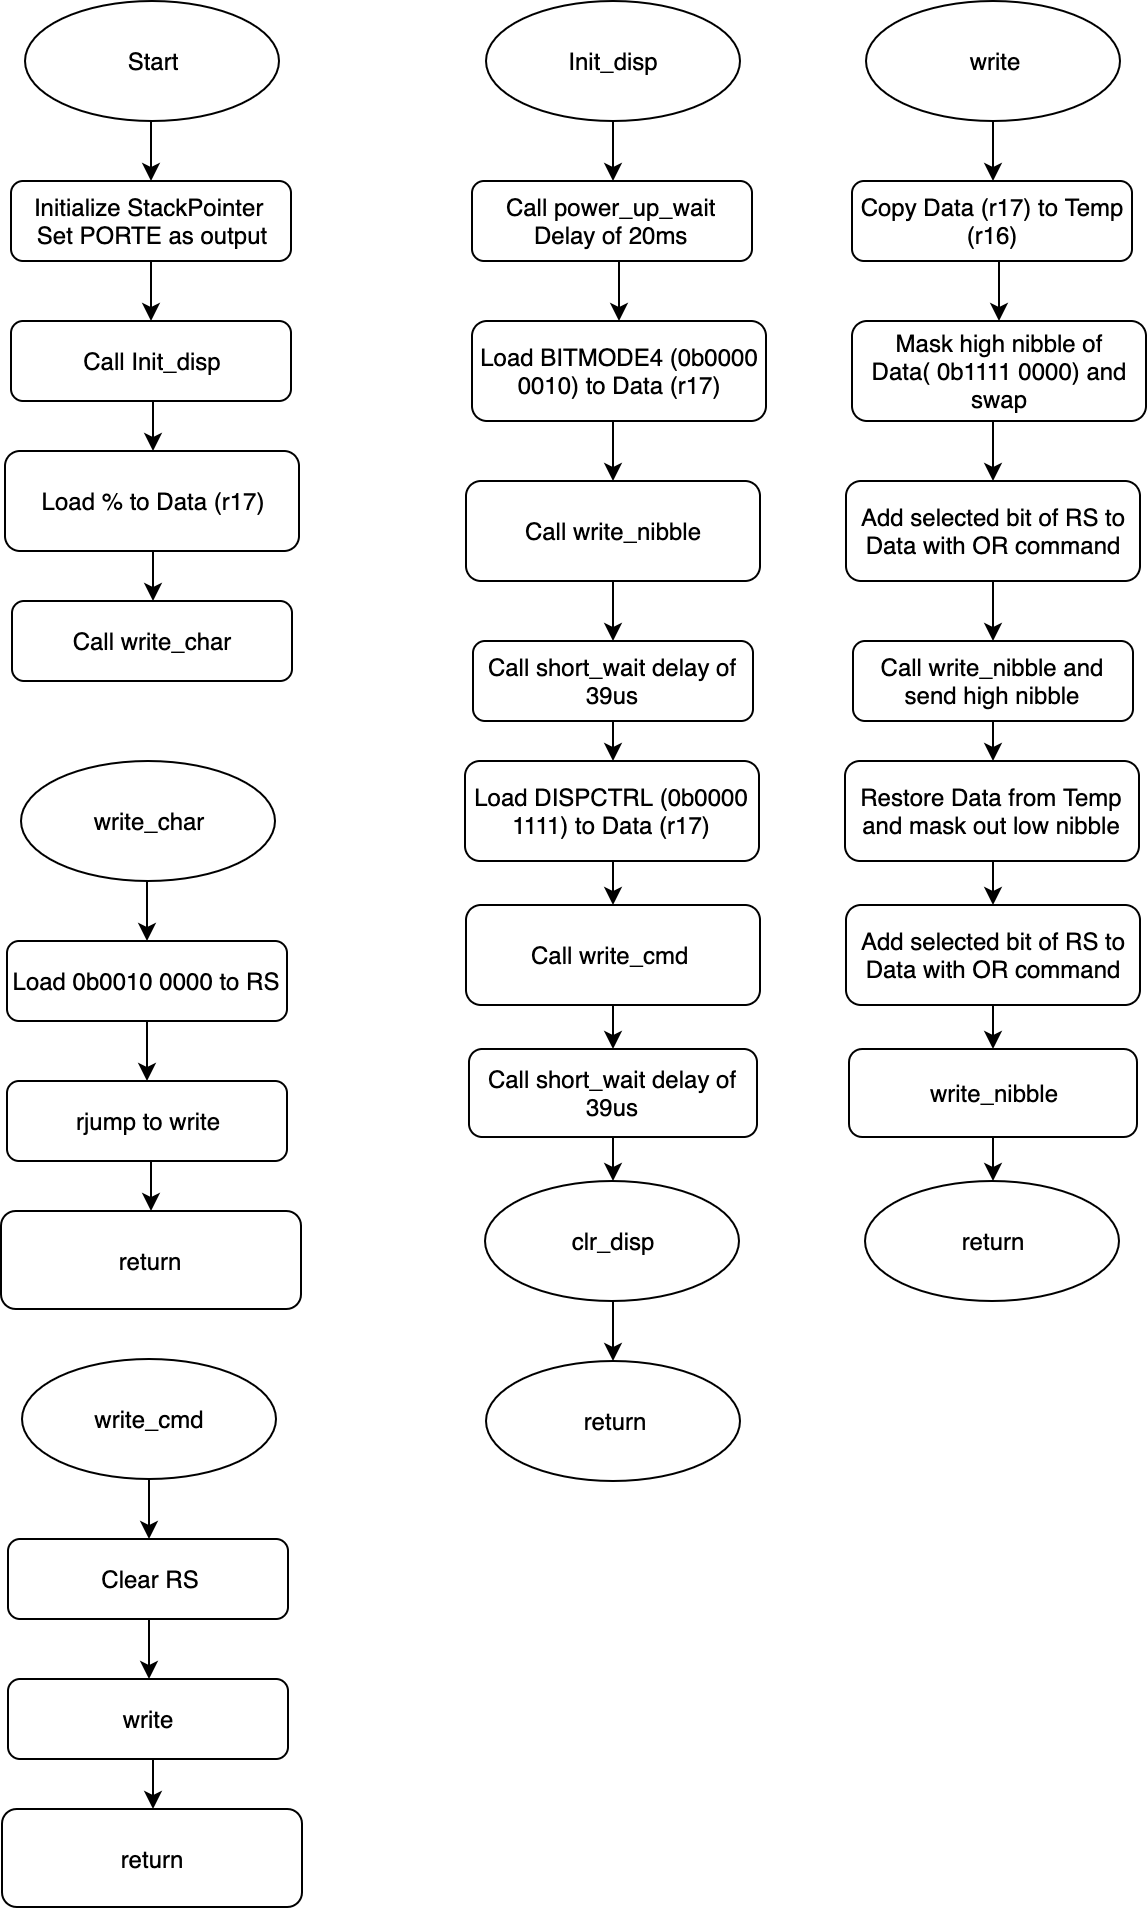
\includegraphics[width=\textwidth/1 ]{flowchart/task1_flowchart.png}
\end{center}
\caption{Task 1 flowchart}
\label{task1}
\end{figure}
\break


%TASK2
\section{Task 2}

\lstset{style=Asm}

\begin{lstlisting}
;>>>>>>>>>>>>>>>>>>>>>>>>>>>>>>>>>>>>>>>>>>>>>>>>>>>>>>>>>>>
; 1DT301, Computer Technology I
; Date: 2016-09-15
; Author:
;	Anas Kwefati
;
; Lab number: 5
; Title: Display JHD202
;
; Hardware: STK600, CPU ATmega2560
;
; Function: Program that generates random numbers between 1 and 75.
;
; Input ports: PORTD Switches (SW0)
;
; Output ports: LCD JHD202 on PORTE.
;
; Subroutines: Interrupt INT0 subroutine
; Included files: m2560def.inc
;
; Other information: The program lab5_init_display.asm was used
; Changes in program: (Description and date)
;<<<<<<<<<<<<<<<<<<<<<<<<<<<<<<<<<<<<<<<<<<<<<<<<<<<<<<<<<<<

.include 	"m2560def.inc"
.def	Temp	= r16
.def	Data	= r17
.def	RS	= r18

.equ	BITMODE4	= 0b00000010		; 4-bit operation
.equ	CLEAR	= 0b00000001			; Clear display
.equ	DISPCTRL	= 0b00001111		; Display on, cursor on, blink on.

.cseg
.org	0x0000				; Reset vector
	jmp reset


.org INT0addr
rjmp interr

.org	0x0072


reset:

	ldi Temp, HIGH(RAMEND)	; Temp = high byte of ramend address
	out SPH, Temp			; sph = Temp
	ldi Temp, LOW(RAMEND)	; Temp = low byte of ramend address
	out SPL, Temp			; spl = Temp

	ser Temp				; r16 = 0b11111111
	out DDRE, Temp			; port E = outputs ( Display JHD202A)
	clr Temp				; r16 = 0
	out PORTE, Temp


	;Main program initialization
	ldi r17, 0x00 ;
	out DDRD, r17 ; we set the DDRD as input

	ldi r17, 0b00000001 ;we set the corresponding bit number to enable the related interrupt here INT0
	out EIMSK, r17 ; Toggle external interrupt requests


	ldi r17, 0b00000010 ;We define the type of signals that activates the external interrupt , here we set it as falling edge to activate the interrupt
	sts EICRA, r17 ;we configure when to switch the external interrupt

	rcall init_disp

	;ASCII CODE : 0x30 == 0 | 0x31 == 1 | 0x39 == 9

	ldi r20, 0x30 ;We load the HEX code 0x31 which is 0 in ASCII code to r20
	;First digit on the LCD

	ldi r21, 0x31 ; r21 is for 2nd digit on the LCD

	ldi Data, 0x31	;We load the HEX code 0x31 which is 1 in ASCII code to Data (r17)

	sei ;enabling all interrupts


loop:

	inc r20 ;Increase r20 by 1
	inc r21 ;second digit increased by 1

	cpi r21, 0x39 ;compare r20 with 0x39 which is 9 in ASCII code
	breq reset_a

	cpi r20, 0x37 ;compare r20 with 0x39 which is 7 in ASCII code
	breq reset_a

	rjmp loop			; loop forever

reset_a :

	ldi r20, 0x30 ;reset r20 to 0
	ldi r21, 0x31 ;reset r20 to 1
	rjmp loop



; **
; ** init_display
; **
init_disp:
	rcall power_up_wait		; wait for display to power up

	ldi Data, BITMODE4		; 4-bit operation
	rcall write_nibble		; (in 8-bit mode)
	rcall short_wait		; wait min. 39 us
	ldi Data, DISPCTRL		; disp. on, blink on, curs. On
	rcall write_cmd			; send command
	rcall short_wait		; wait min. 39 us
clr_disp:
	ldi Data, CLEAR			; clr display
	rcall write_cmd			; send command
	rcall long_wait			; wait min. 1.53 ms
	ret

; **
; ** write char/command
; **

write_char:
	ldi RS, 0b00100000		; RS = high
	rjmp write
write_cmd:
	clr RS					; RS = low
write:
	mov Temp, Data			; copy Data
	andi Data, 0b11110000	; mask out high nibble
	swap Data				; swap nibbles
	or Data, RS				; add register select
	rcall write_nibble		; send high nibble
	mov Data, Temp			; restore Data
	andi Data, 0b00001111	; mask out low nibble
	or Data, RS				; add register select

write_nibble:
	rcall switch_output		; Modify for display JHD202A, port E
	nop						; wait 542nS
	sbi PORTE, 5			; enable high, JHD202A
	nop
	nop						; wait 542nS
	cbi PORTE, 5			; enable low, JHD202A
	nop
	nop						; wait 542nS
	ret

; **
; ** busy_wait loop
; **
short_wait:
	clr zh					; approx 50 us
	ldi zl, 30
	rjmp wait_loop
long_wait:
	ldi zh, HIGH(1000)		; approx 2 ms
	ldi zl, LOW(1000)
	rjmp wait_loop
dbnc_wait:
	ldi zh, HIGH(4600)		; approx 10 ms
	ldi zl, LOW(4600)
	rjmp wait_loop
power_up_wait:
	ldi zh, HIGH(9000)		; approx 20 ms
	ldi zl, LOW(9000)

wait_loop:
	sbiw z, 1				; 2 cycles
	brne wait_loop			; 2 cycles
	ret

; **
; ** modify output signal to fit LCD JHD202A, connected to port E
; **

switch_output:
	push Temp
	clr Temp
	sbrc Data, 0				; D4 = 1?
	ori Temp, 0b00000100		; Set pin 2
	sbrc Data, 1				; D5 = 1?
	ori Temp, 0b00001000		; Set pin 3
	sbrc Data, 2				; D6 = 1?
	ori Temp, 0b00000001		; Set pin 0
	sbrc Data, 3				; D7 = 1?
	ori Temp, 0b00000010		; Set pin 1
	sbrc Data, 4				; E = 1?
	ori Temp, 0b00100000		; Set pin 5
	sbrc Data, 5				; RS = 1?
	ori Temp, 0b10000000		; Set pin 7 (wrong in previous version)
	out porte, Temp
	pop Temp
	ret



;Interrupt

interr :

	cpi r20, 0x37; compare the 1st digit with the number 7
	breq check ;if r20 == 7 we go to check
	;We do this to make sure that it will never go more than 7 for the first digit
	;because the maximum number is 75
	brne normal ; otherwise normal

	check :
		rcall clr_disp ;call clear display

		mov Data, r20
		;ldi Data, 0x31
		;add Data, r20
		rcall write_char ;print the first digit 7

		;CHECK IF r21 >= 5
		cpi r21, 0x35 ;5
		brge resetr ;if r21 (2nd digit) >= 5 go to resetr

		resetr:
			rcall clr_disp ;call clear display
			mov Data, r21
			rcall short_wait
			rcall write_char
			RETI ;End of interrupt



	normal :

		;DISPLAY NUMBERS
		rcall clr_disp ;call clear display

		mov Data, r20
		rcall write_char

		mov Data, r21
		rcall short_wait
		rcall write_char

RETI ;End of Interrupt

\end{lstlisting}

\begin{figure}
\begin{center}
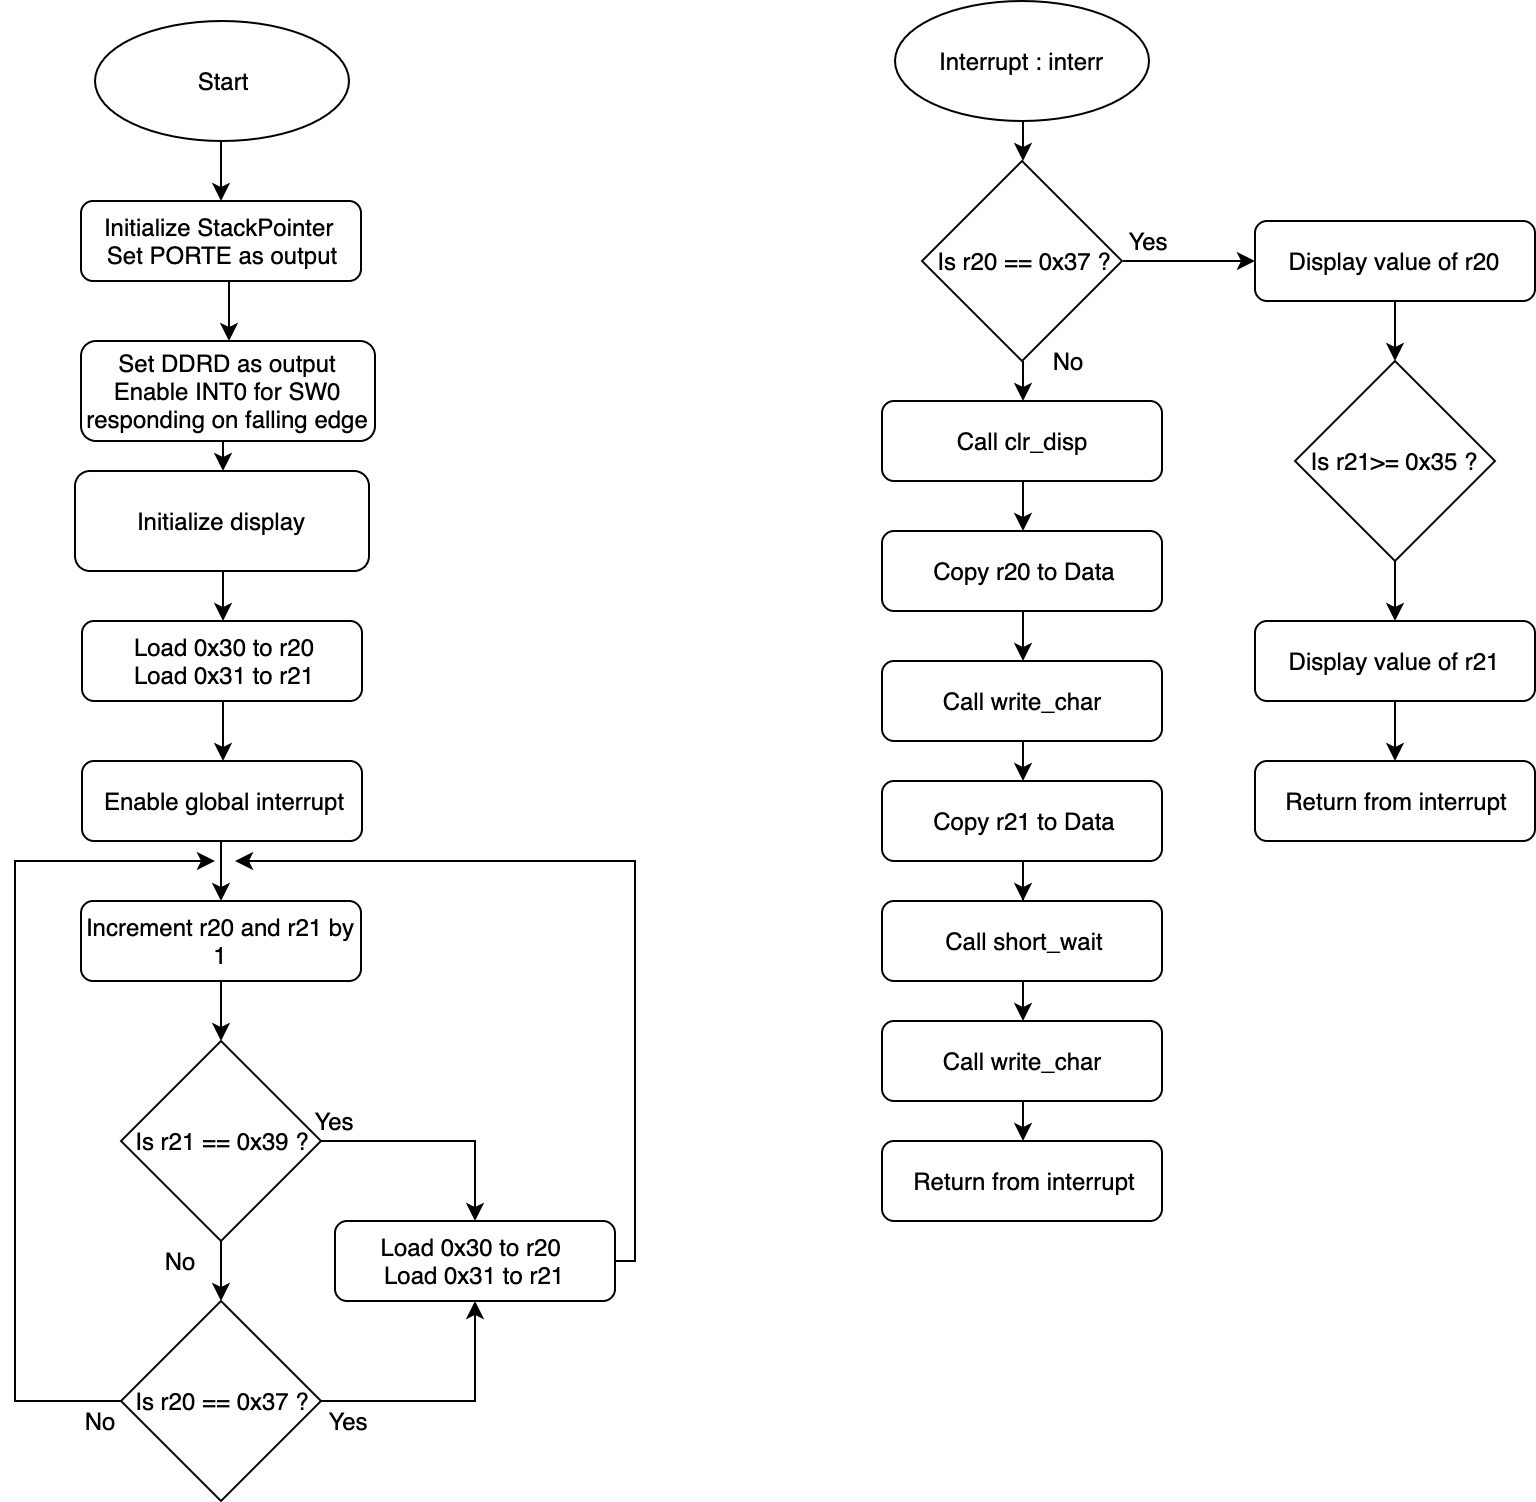
\includegraphics[width=\textwidth/1]{flowchart/task2_flowchart.png}
\end{center}
\caption{Task 2 flowchart}
\label{task2}
\end{figure}




%TASK 3
\break
\section{Task 3}

\lstset{style=Asm}

\begin{lstlisting}
;>>>>>>>>>>>>>>>>>>>>>>>>>>>>>>>>>>>>>>>>>>>>>>>>>>>>>>>>>>>
; 1DT301, Computer Technology I
; Date: 2016-09-15
; Author:
;	Anas Kwefati
;
; Lab number: 5
; Title: Display JHD202
;
; Hardware: STK600, CPU ATmega2560
;
; Function: Program that receives a character on the serial port and displays
; each character on the display JHD202
;
; Input ports: PORT0 (RS232) VGA
;
; Output ports: LCD JHD202 on PORTE and LEDs on PORTB
;
; Subroutines:
; Included files: m2560def.inc
;
; Other information: The program lab5_init_display.asm was used
; task 3 from lab4 was also used
; Changes in program: (Description and date)
;<<<<<<<<<<<<<<<<<<<<<<<<<<<<<<<<<<<<<<<<<<<<<<<<<<<<<<<<<<<
.include 	"m2560def.inc"
.def	Temp	= r16
.def	Data	= r17
.def	RS	= r18

.equ	BITMODE4	= 0b00000010		; 4-bit operation
.equ	CLEAR	= 0b00000001			; Clear display
.equ	DISPCTRL	= 0b00001111		; Display on, cursor on, blink on.

.cseg
.org	0x0000				; Reset vector
	jmp reset


.org	0x0072

reset:

	ldi Temp, HIGH(RAMEND)	; Temp = high byte of ramend address
	out SPH, Temp			; sph = Temp
	ldi Temp, LOW(RAMEND)	; Temp = low byte of ramend address
	out SPL, Temp			; spl = Temp

	ser Temp				; r16 = 0b11111111
	out DDRE, Temp			; port E = outputs ( Display JHD202A)
	clr Temp				; r16 = 0
	out PORTE, Temp


	;Main program initialization
	ldi r16,0xFF	;PORTB outputs
	out DDRB, r16

	out PORTB, r16

	;We initialize for the serial communication PORT0(RS232)
	ldi r19, 12	;osc = 1MHz, 4800 bps => UBBRR = 12
	sts UBRR1L , r19	;Store Prescaler value in UBRR1L

	ldi r19, (1<<RXEN1)	;Set RX enable flags
	sts UCSR1B, r19

	rcall init_disp ;call init_disp

	sei ;enabling all interrupts


GetChar:	;Receive data
	lds r19, UCSR1A	;read UCSR1A I/0 register to r16
	sbrs r19,RXC1	;RXC1=1 -> new Character Skip if bit RXC1 is set in r16
	rjmp GetChar	;RXC1=0 -> no character received otherwise rjmp
	lds r23,UDR1	;Read character in UDR

Port_output:	;Show data on the LEDs
	mov Data, r23 ;put the value of r23 to Data (r17)
	out PORTB, r23 ;output LEDs
	rcall write_char	;Write character to PORTE (LCD)

rjmp GetChar ;rjump to the beginning


; **
; ** init_display
; **
init_disp:
	rcall power_up_wait		; wait for display to power up

	ldi Data, BITMODE4		; 4-bit operation
	rcall write_nibble		; (in 8-bit mode)
	rcall short_wait		; wait min. 39 us
	ldi Data, DISPCTRL		; disp. on, blink on, curs. On
	rcall write_cmd			; send command
	rcall short_wait		; wait min. 39 us
clr_disp:
	ldi Data, CLEAR			; clr display
	rcall write_cmd			; send command
	rcall long_wait			; wait min. 1.53 ms
	ret

; **
; ** write char/command
; **

write_char:
	ldi RS, 0b00100000		; RS = high
	rjmp write
write_cmd:
	clr RS					; RS = low
write:
	mov Temp, Data			; copy Data
	andi Data, 0b11110000	; mask out high nibble
	swap Data				; swap nibbles
	or Data, RS				; add register select
	rcall write_nibble		; send high nibble
	mov Data, Temp			; restore Data
	andi Data, 0b00001111	; mask out low nibble
	or Data, RS				; add register select

write_nibble:
	rcall switch_output		; Modify for display JHD202A, port E
	nop						; wait 542nS
	sbi PORTE, 5			; enable high, JHD202A
	nop
	nop						; wait 542nS
	cbi PORTE, 5			; enable low, JHD202A
	nop
	nop						; wait 542nS
	ret

; **
; ** busy_wait loop
; **
short_wait:
	clr zh					; approx 50 us
	ldi zl, 30
	rjmp wait_loop
long_wait:
	ldi zh, HIGH(1000)		; approx 2 ms
	ldi zl, LOW(1000)
	rjmp wait_loop
dbnc_wait:
	ldi zh, HIGH(4600)		; approx 10 ms
	ldi zl, LOW(4600)
	rjmp wait_loop
power_up_wait:
	ldi zh, HIGH(9000)		; approx 20 ms
	ldi zl, LOW(9000)

wait_loop:
	sbiw z, 1				; 2 cycles
	brne wait_loop			; 2 cycles
	ret

; **
; ** modify output signal to fit LCD JHD202A, connected to port E
; **

switch_output:
	push Temp
	clr Temp
	sbrc Data, 0				; D4 = 1?
	ori Temp, 0b00000100		; Set pin 2
	sbrc Data, 1				; D5 = 1?
	ori Temp, 0b00001000		; Set pin 3
	sbrc Data, 2				; D6 = 1?
	ori Temp, 0b00000001		; Set pin 0
	sbrc Data, 3				; D7 = 1?
	ori Temp, 0b00000010		; Set pin 1
	sbrc Data, 4				; E = 1?
	ori Temp, 0b00100000		; Set pin 5
	sbrc Data, 5				; RS = 1?
	ori Temp, 0b10000000		; Set pin 7 (wrong in previous version)
	out porte, Temp
	pop Temp
	ret


\end{lstlisting}

\begin{figure}
\begin{center}
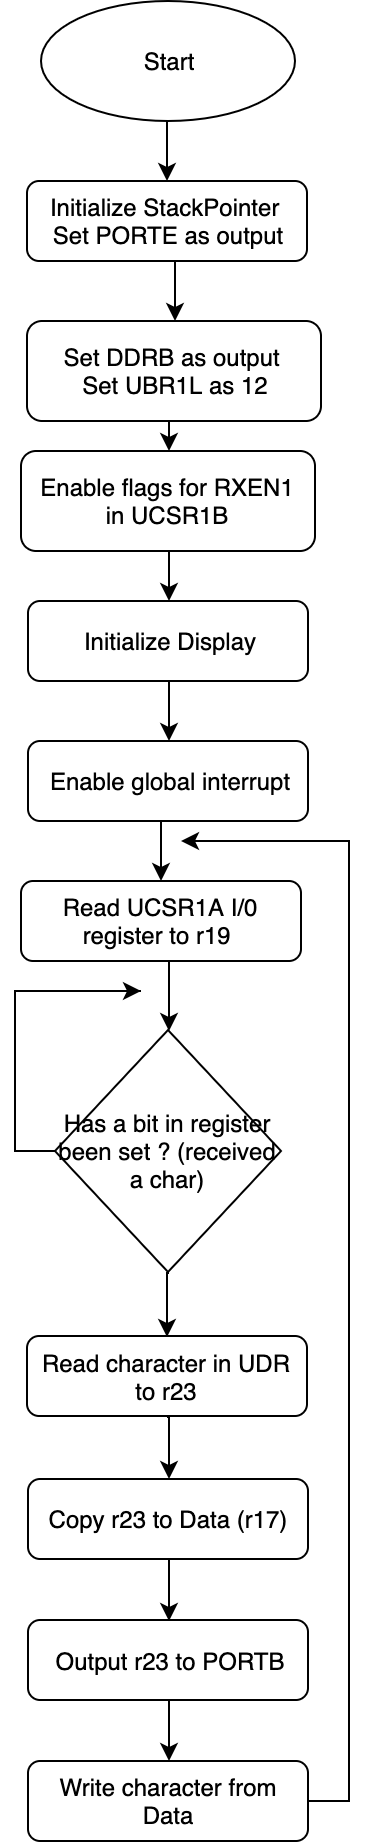
\includegraphics[width=\textwidth/4 ]{flowchart/task3_flowchart.png}
\end{center}
\caption{Task 3 flowchart}
\label{task3}
\end{figure}

\break

%TASK4
\section{Task 4}

\lstset{style=Asm}

\begin{lstlisting}
;>>>>>>>>>>>>>>>>>>>>>>>>>>>>>>>>>>>>>>>>>>>>>>>>>>>>>>>>>>>
; 1DT301, Computer Technology I
; Date: 2016-09-15
; Author:
;	Anas Kwefati
;
; Lab number: 5
; Title: Display JHD202
;
; Hardware: STK600, CPU ATmega2560
;
; Function: Program that takes 4 lines of text. Each textline should be
; displayed during 5 seconds, after that the text on line 1 should be moved to
; line 2 and so on. The text is entered from the terminal program PUTTY via serial port
;
; Input ports: PORT0 (RS232) VGA
;
; Output ports: LCD JHD202 on PORTE.
;
; Subroutines:
; Included files: m2560def.inc
;
; Other information: The program lab5_init_display.asm was used
; task 3 from lab4 was also used and task 3 from lab5
; Changes in program: (Description and date)
;<<<<<<<<<<<<<<<<<<<<<<<<<<<<<<<<<<<<<<<<<<<<<<<<<<<<<<<<<<<

.include 	"m2560def.inc"
.def	Temp	= r16
.def	Data	= r17
.def	RS	= r25
.def	COUNTER = r24


.equ	BITMODE4	= 0b00000010		; 4-bit operation
.equ	CLEAR	= 0b00000001			; Clear display
.equ	DISPCTRL	= 0b00001111		; Display on, cursor on, blink on.

.cseg
.org	0x0000				; Reset vector
	jmp reset

.org URXC1addr	;USART Interrupt
rjmp GetChar

.org	0x0072

reset:
	ldi COUNTER,0
	ldi Temp, HIGH(RAMEND)	; Temp = high byte of ramend address
	out SPH, Temp			; sph = Temp
	ldi Temp, LOW(RAMEND)	; Temp = low byte of ramend address
	out SPL, Temp			; spl = Temp

	ser Temp				; r16 = 0b11111111
	out DDRE, Temp			; port E = outputs ( Display JHD202A)
	clr Temp				; r16 = 0
	out PORTE, Temp

	ldi r16,0xFF
	out DDRB,r16

	out PORTB,r16

	ldi r19, 12		;osc = 1MHz, 4800 bps => UBBRR = 12
	sts UBRR1L , r19	;Store Prescaler value in UBRR1L

	ldi r19, (1<<RXEN1 | 1<<TXEN1);Set RX, TX enable flags and RXCIE = 1
	sts UCSR1B, r19


	;We set the registers at the address 0x200
	;The idea is to be able to store the data into the internal memory
	ldi YH, HIGH (0x200)
	ldi YL, LOW(0x200)
	ldi XH, HIGH (0x200)
	ldi XL, LOW(0x200)

	rcall init_disp ;call init_disp

	sei	;Set global interrupt flag

GetChar:	;Receive data
	lds r21, UCSR1A	;read UCSR1A I/0 register to r21
	sbrs r21,RXC1	;RXC1=1 -> new Character Skip if bit RXC1 is set in r21
	rjmp GetChar	;RXC1=0 -> no character received otherwise rjmp
	lds r23,UDR1	;Read character in UDR

	cpi r23, 0x0D ; compare r23 with ASCII code return line carriage return
	breq nextLine ;if yes go to nextLine
	st Y+,r23 ;store indirect from register to data space using Index Y
	;so we store r23 to data space using Index Y

	Port_output:
		mov Data, r23 ;put the value of r23 to Data (r17)
		out PORTB, r23 ;output LEDs
		rcall write_char	;Write character to PORTE (LCD)

	PutChar:
		lds r21, UCSR1A	;Read UCSR1A i/O register to r20
		sbrs r21, UDRE1	;UDRE1 =1 => buffer is empty
		rjmp PutChar	;UDRE1 = 0 => buffer is not empty
		sts UDR1,r23	;write character to UDR1
		rjmp something

	nextLine:
		rcall delay;we call delay to wait 5s
		ldi Data, CLEAR ;clear everything on the LCD
		rcall write_cmd
		rcall long_wait

		ldi Data, 0x40 ;we go to the line
		rcall write_cmd

			loop:
				;we compare before we get out of boundary in the memory
				cp YH , XH ;we compare YHighest with XH
				brne print ;if not equal go to print
				cp YL , XL ;compare Lowest value of YL and XL
				breq stop_print ;if it is equal go to stop print

				print:
					ld Data, X+ ;Load Indirect from data space to register using Index X
					;we load value in X+ to Data
					rcall write_char
					rcall long_wait
					rjmp loop

			stop_print:
				;we reset the values
				ldi YH, HIGH (0x200)
				ldi YL, LOW(0x200)
				ldi XH, HIGH (0x200)
				ldi XL, LOW(0x200)
				ldi Data, 0b00000010
				rcall write_cmd

				rjmp something

something:
	nop
rjmp GetChar	;Return to GetChar


clr_disp:
	ldi Data, CLEAR			; clr display
	rcall write_cmd			; send command
	rcall long_wait			; wait min. 1.53 ms
	ret

; **
; ** write char/command
; **

write_char:
	ldi RS, 0b00100000		; RS = high
	rjmp write
write_cmd:
	clr RS					; RS = low
write:
	mov Temp, Data			; copy Data
	andi Data, 0b11110000	; mask out high nibble
	swap Data				; swap nibbles
	or Data, RS				; add register select
	rcall write_nibble		; send high nibble
	mov Data, Temp			; restore Data
	andi Data, 0b00001111	; mask out low nibble
	or Data, RS				; add register select

write_nibble:
	rcall switch_output		; Modify for display JHD202A, port E
	nop						; wait 542nS
	sbi PORTE, 5			; enable high, JHD202A
	nop
	nop						; wait 542nS
	cbi PORTE, 5			; enable low, JHD202A
	nop
	nop						; wait 542nS
	ret

; **
; ** busy_wait loop
; **
short_wait:
	clr zh					; approx 50 us
	ldi zl, 30
	rjmp wait_loop
long_wait:
	ldi zh, HIGH(1000)		; approx 2 ms
	ldi zl, LOW(1000)
	rjmp wait_loop
dbnc_wait:
	ldi zh, HIGH(4600)		; approx 10 ms
	ldi zl, LOW(4600)
	rjmp wait_loop
power_up_wait:
	ldi zh, HIGH(9000)		; approx 20 ms
	ldi zl, LOW(9000)

wait_loop:
	sbiw z, 1				; 2 cycles
	brne wait_loop			; 2 cycles
	ret

; **
; ** modify output signal to fit LCD JHD202A, connected to port E
; **

switch_output:
	push Temp
	clr Temp
	sbrc Data, 0				; D4 = 1?
	ori Temp, 0b00000100		; Set pin 2
	sbrc Data, 1				; D5 = 1?
	ori Temp, 0b00001000		; Set pin 3
	sbrc Data, 2				; D6 = 1?
	ori Temp, 0b00000001		; Set pin 0
	sbrc Data, 3				; D7 = 1?
	ori Temp, 0b00000010		; Set pin 1
	sbrc Data, 4				; E = 1?
	ori Temp, 0b00100000		; Set pin 5
	sbrc Data, 5				; RS = 1?
	ori Temp, 0b10000000		; Set pin 7 (wrong in previous version)
	out porte, Temp
	pop Temp
	ret

delay:
	; Generated by delay loop calculator
	; at http://www.bretmulvey.com/avrdelay.html
	; Delay 9 215 000 cycles
	; 5s at 1.843 MHz
	    ldi  r18, 47
	    ldi  r19, 192
	    ldi  r20, 104
	L1: dec  r20
	    brne L1
	    dec  r19
	    brne L1
	    dec  r18
	    brne L1
	RET

\end{lstlisting}
\break
\begin{figure}
\begin{center}
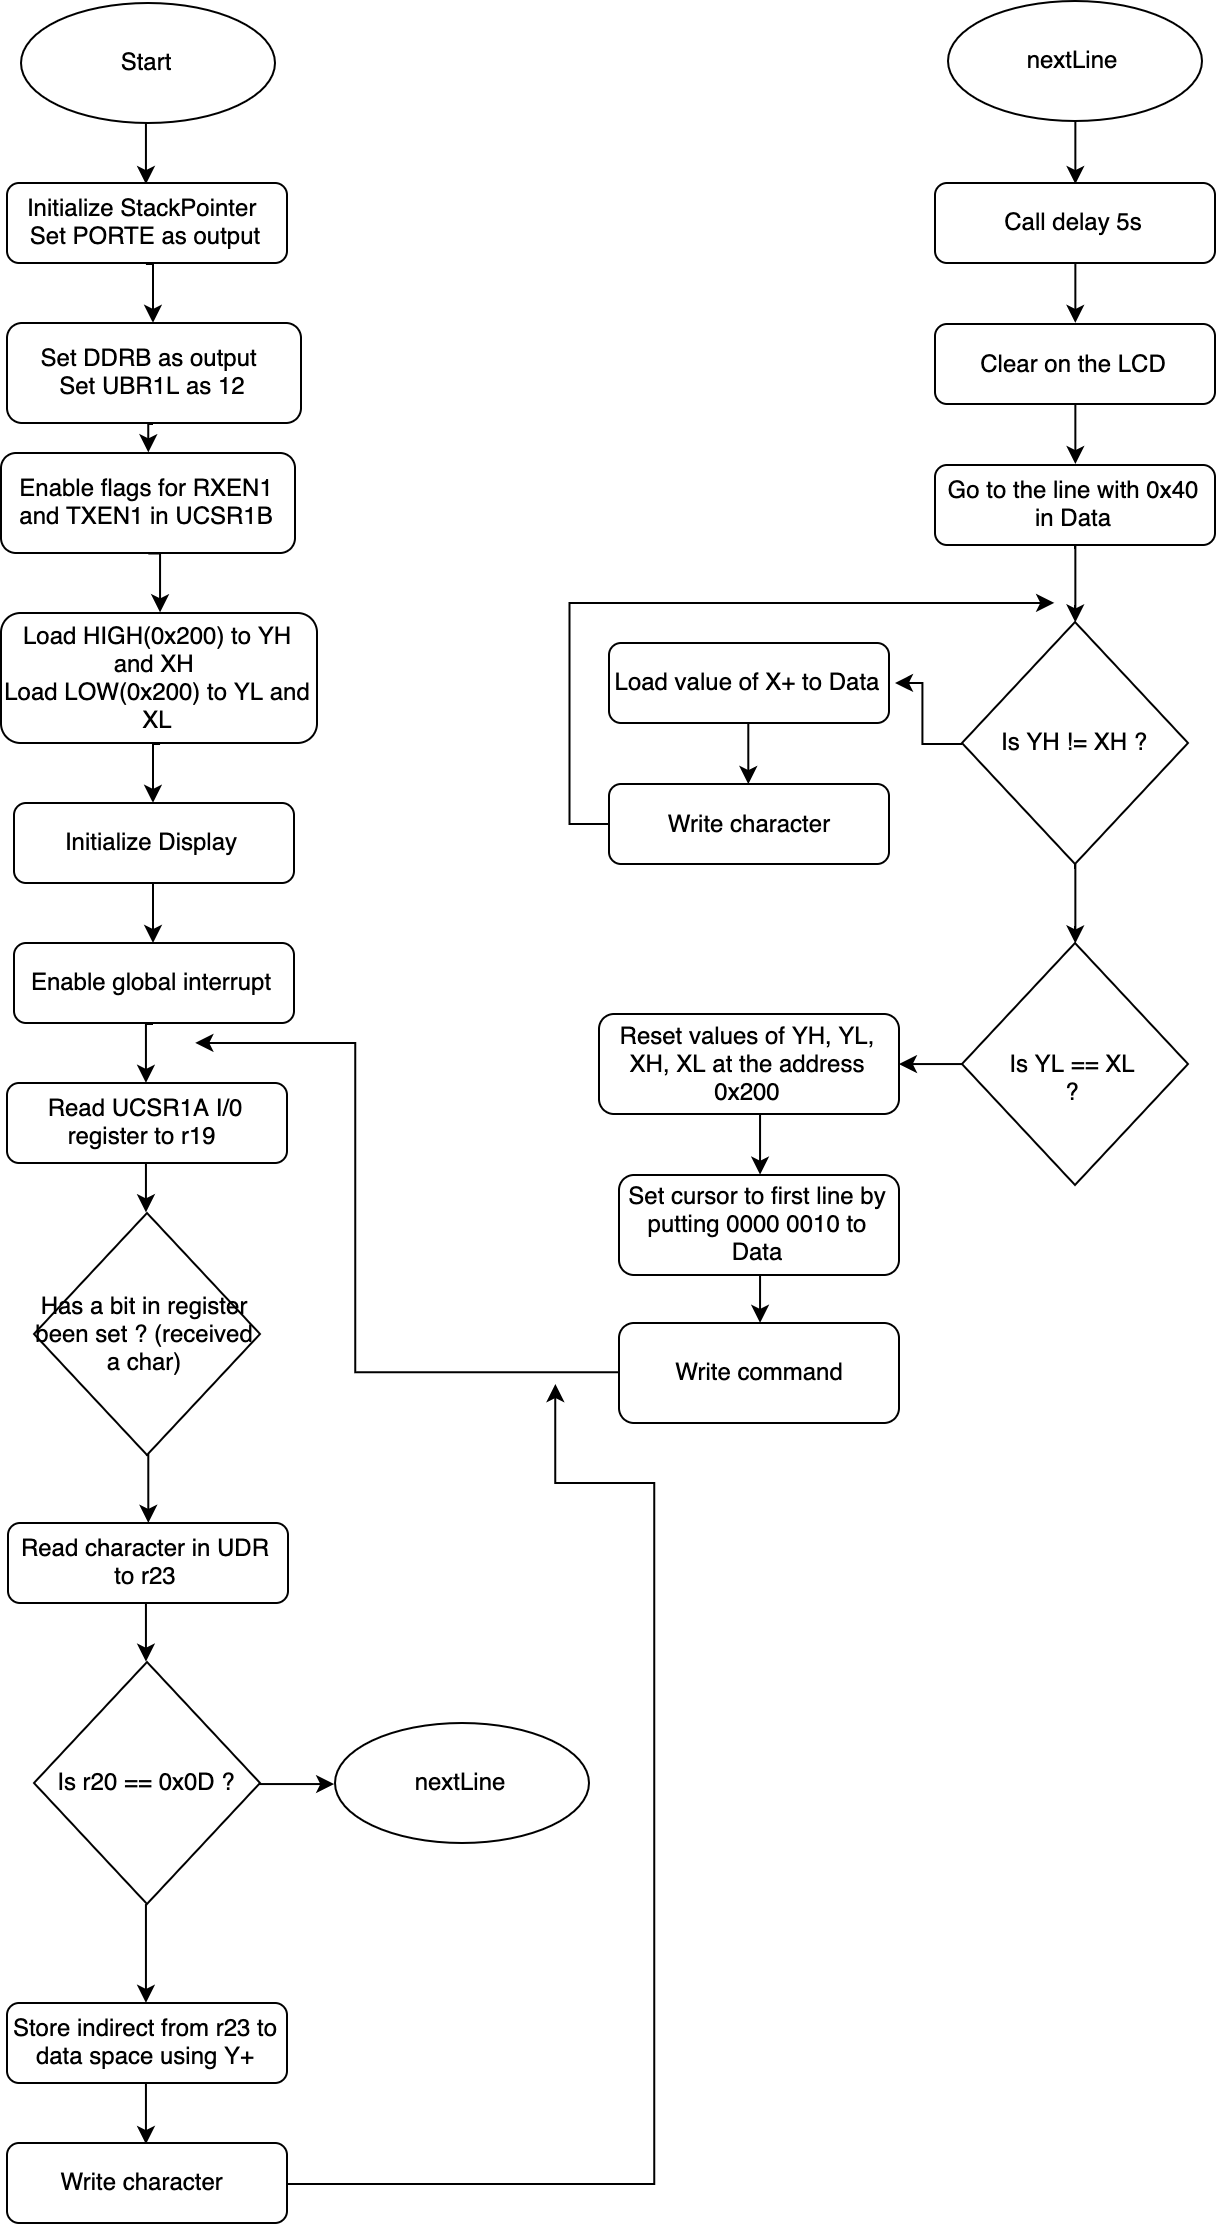
\includegraphics[width=\textwidth/1 ]{flowchart/task4_flowchart.png}
\end{center}
\caption{Task 4 flowchart}
\label{task4}
\end{figure}




% Prints your bibliography database xxx.bib
\bibliographystyle{IEEEtran}
\bibliography{ref.bib}

\end{document}
